\section{SEDflow} \label{sec:sedflow}
%The goal of this work is to demonstrate that we can exploit ANPE to accelerate Bayesian SED modeling.  
In this section, we present \sedflow, which applies ANPE to SED modeling for a
scalable and accelerated approach.
For our SED model, we use the state-of-the-art PROVABGS model from
\cite{hahn2022}. 
Although many SED models have been recently used in the
literature~(\emph{e.g.} {\sc Bagpipes}, \citealt{carnall2018}; 
{\sc Prospector}, \citealt{leja2017, johnson2021}), we choose PROVABGS because
it will be used to analyze >10 million galaxy spectrophotometry measured by the
DESI Bright Galaxy Survey~\citep{ruiz-macias2021, hahn2022}.
Below, we describe the PROVABGS model, the construction of the
\sedflow~training data using PROVABGS, and the training procedure for \sedflow.

% section explaining specific SED set up 
\subsection{SED Modeling: PROVABGS} \label{sec:provabgs}
We use the state-of-the-art SPS model of the
PROVABGS~(\chedit{Hahn~\etal~2022}). 
The SED of a galaxy is modeled as a composite of stellar populations defined by
stellar evolution theory (in the form of isochrones, stellar spectral
libraries, and an initial mass function) and its star
formation and chemical enrichment histories (SFH and ZH), attenuated by
dust~\citep[see][for a review]{walcher2011, conroy2013}. 
The PROVABGS model, in particular, utilizes a non-parametric SFH with a
starburst, a non-parametric ZH that varies with time, and a flexible dust
attenuation prescription.

% highlight advantages of provabgs 
The SFH has two components: one based on non-negative matrix factorization
(NMF) bases and the other, a starburst component.
The SFH contribution from the NMF component is a linear combination of four NMF
SFH basis functions, derived from performing NMF~\citep{lee1999, cichocki2009,
fevotte2011} on SFHs of galaxies in the Illustris cosmological hydrodynamical
simulations~\citep{vogelsberger2014, genel2014, nelson2015}.
The NMF SFH prescription provides a compact and flexible representation of the
SFH.
The second starburst component consists of a single stellar population (SSP)
and adds stochasticity to the SFH. 

The ZH is similar defined using two NMF bases dervied from Illustris. 
This ZH prescription enables us to flexibly model a wide range of ZHs and
unlike most SED models, it does not assume constant metallicity over time, whichcan significantly bias inferred galaxy properties~\citep{thorne2021}. 
The stellar evolution theory is based on Flexible Stellar Population
Synthesis~\citep[FSPS;][]{conroy2009, conroy2010c} with the MIST
isochrones~\citep{paxton2011, paxton2013, paxton2015, choi2016, dotter2016},  
the \cite{chabrier2003} initial mass function (IMF), and a combination of the
MILES~\citep{sanchez-blazquez2006} and BaSeL~\citep{lejeune1997, lejeune1998,
westera2002} libraries.
The SFH and ZH are binned into 43 logarithmically-space time bin and SSPs are
evalulated at each time bin using FSPS. 
The SSPs are summed up to get the unattenuated rest-frame galaxy SED. 

Lastly, PROVABGS attenuates the light from the composite stellar population
using the two component \cite{charlot2000} dust attenuation model with
diffuse-dust (ISM) and birth cloud (BC) components. 
All SSPs are attenuated by the diffuse dust using the \cite{kriek2013}
attenuation curve.
Then, the BC component provides extra dust attenuation on SSPs younger than 100
Myr with young stars that are embedded in modecular clouds and HII regions. 
In total the PROVABGS SED model has 12 free parameters: stellar mass ($M_*$),
six SFH parameters ($\beta_1, \beta_2, \beta_3, \beta_4, t_{\rm burst}, f_{\rm
burst}$), two ZH parameters ($\gamma_1, \gamma2$), and three dust attenuation
parameters ($\tau_{\rm BC}, \tau_{\rm ISM}, n_{\rm dust}$). 
Each PROVABGS model evaluation takes ${\sim}340$ ms. 


\begin{figure}
\begin{center}
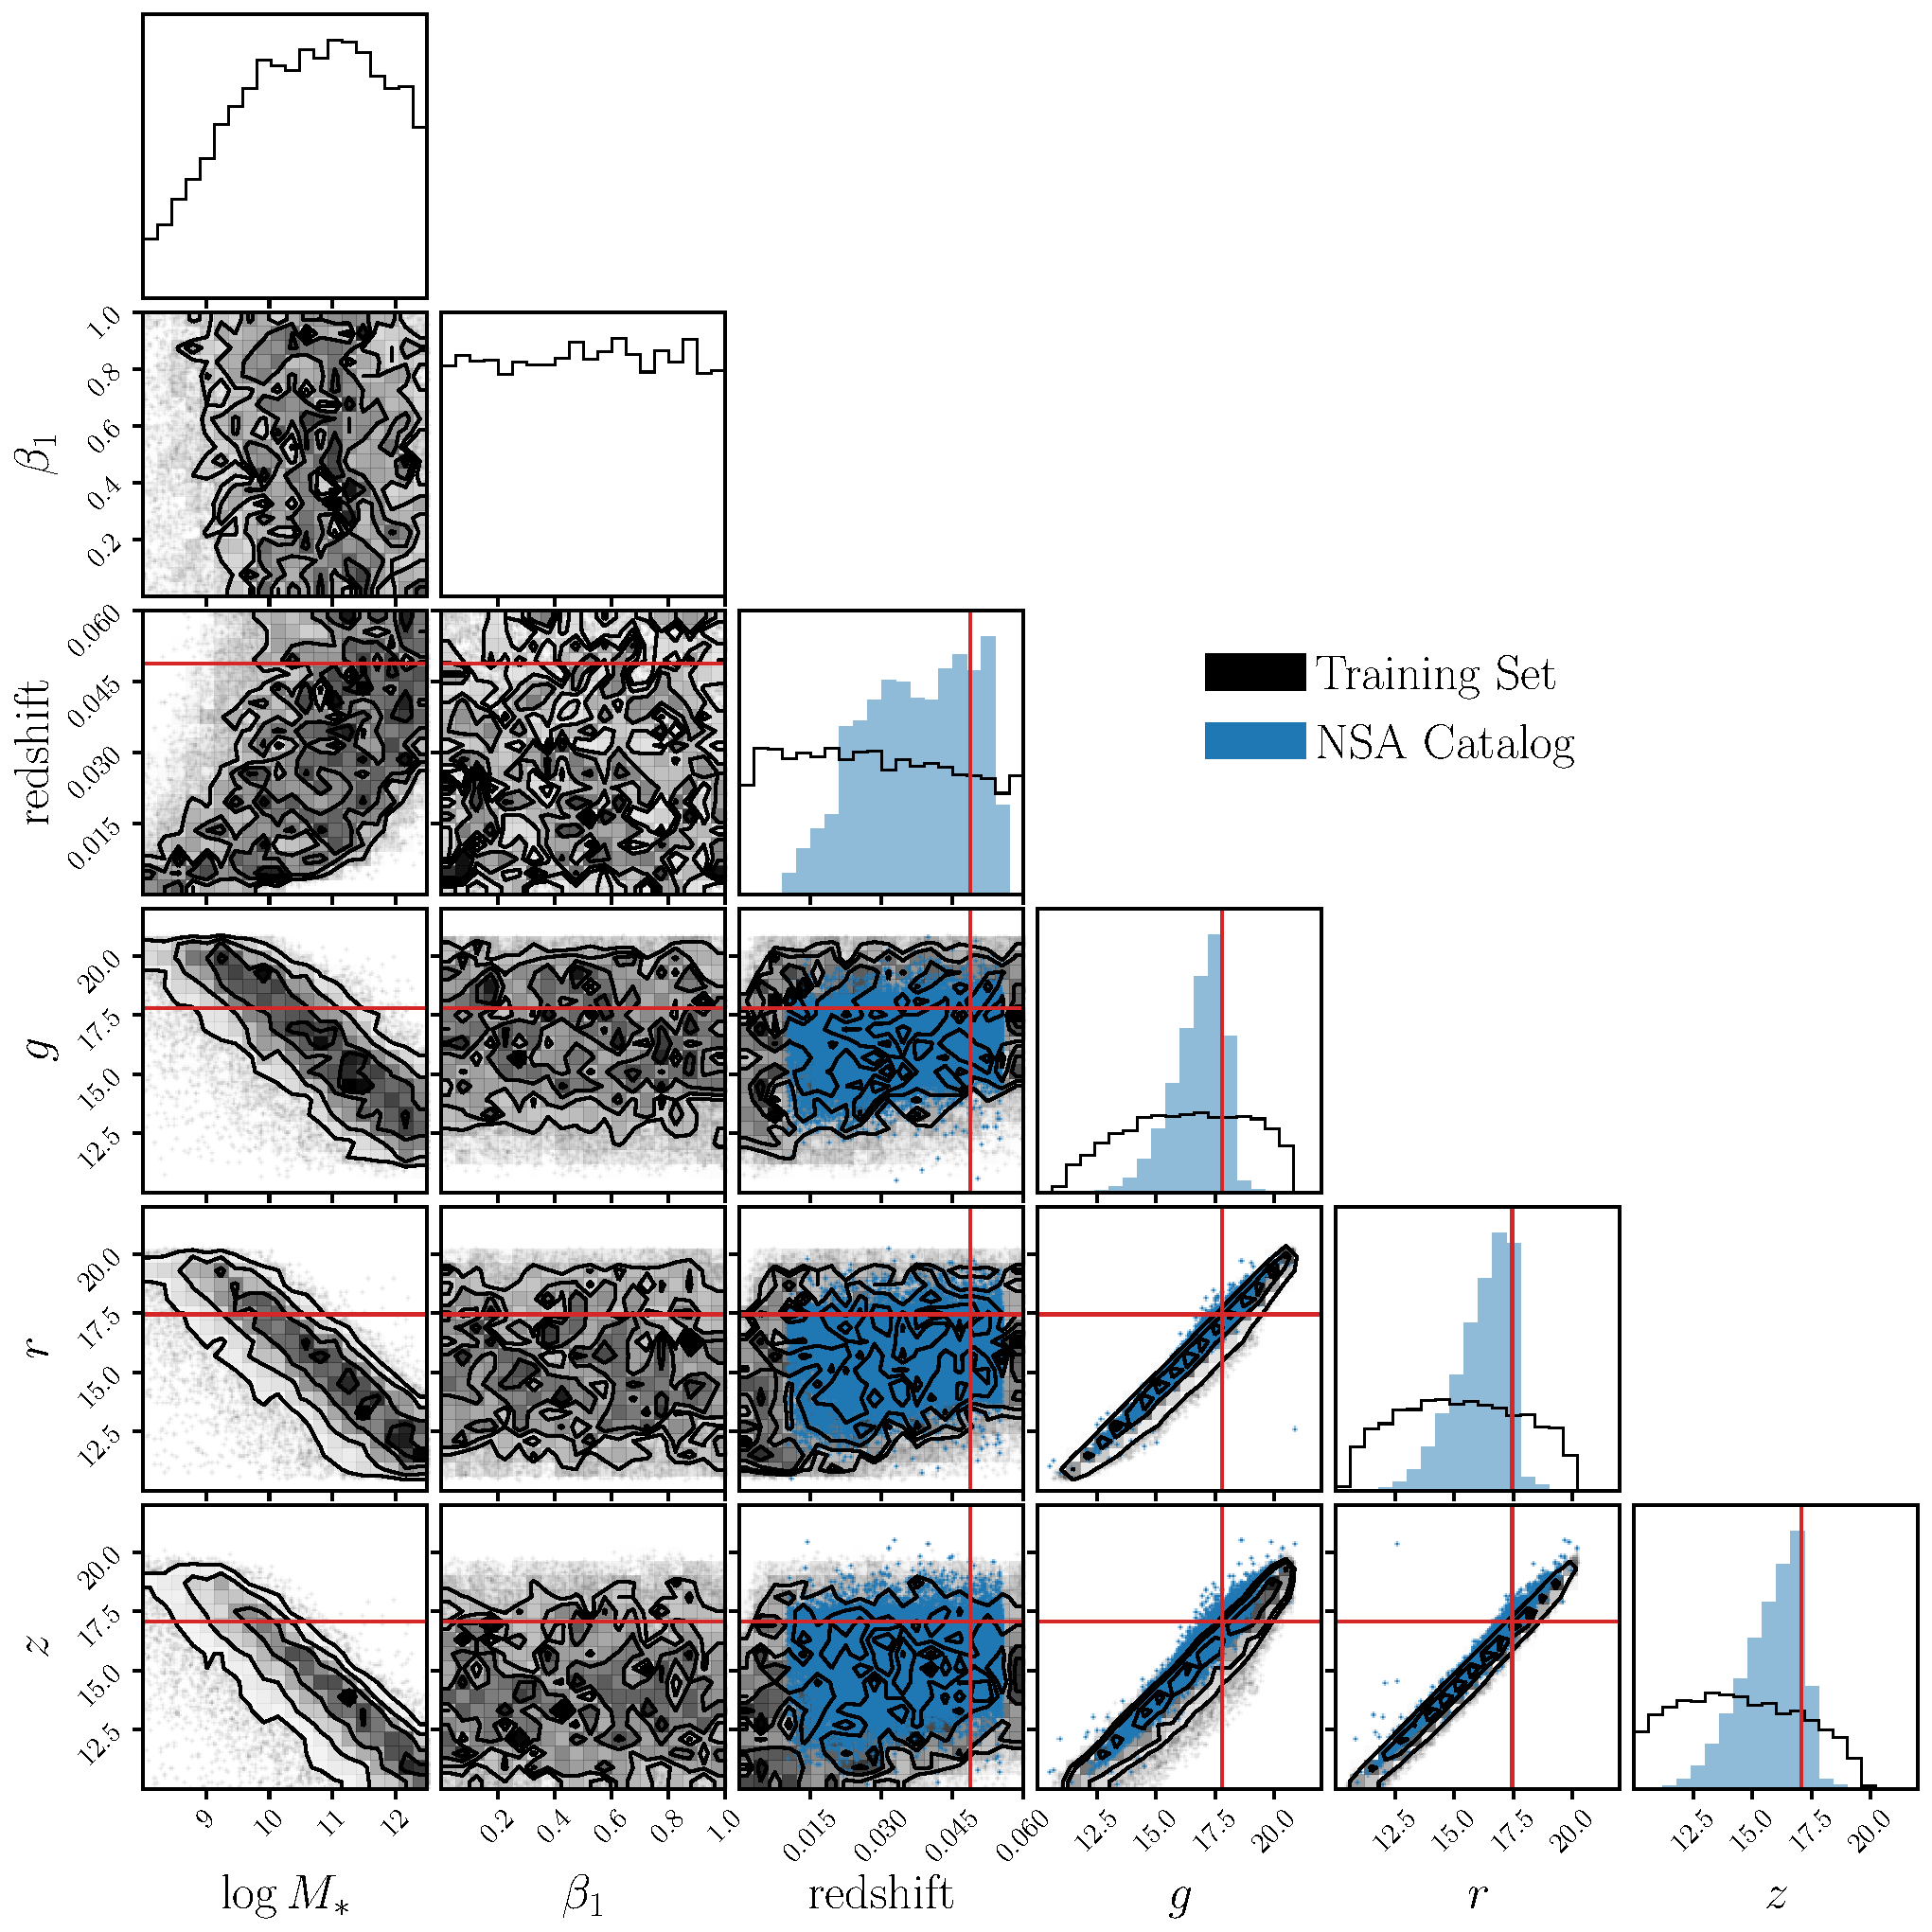
\includegraphics[width=0.9\textwidth]{figs/training.pdf}
    \caption{\label{fig:data}
    Joint distribution of SED model parameters, redshift, photometric
    magnitudes, and uncertainties of the data used to train \sedflow.
    We plot only a subset of the parameters ($\log M_*$, $\beta_1$) and
    photometric bands for clarity.
    The training data was constructed by sampling SED model parameter values
    from the prior and forward modeling optical photometry using the PROVABGS
    and noise models (Section~\ref{sec:sedflow}). 
    For comparison, we present the distribution of redshift, magnitudes, and
    uncertainties for galaxies in the NSA catalog (blue). 
    \emph{The training set fully encompasses the observations; thus, 
    {\sc SEDflow} can be used to infer the posterior for all NSA galaxies}.
    }
\end{center}
\end{figure}
%%%%%%%%%%%%%%%%%%%%%%%%%%%%%%%%%%%%%%%%%%%%%%%%%%%%%%%%%%%%%%%%%%%%%%%%%%%%
% training data 
%%%%%%%%%%%%%%%%%%%%%%%%%%%%%%%%%%%%%%%%%%%%%%%%%%%%%%%%%%%%%%%%%%%%%%%%%%%%
\subsection{Training Data} \label{sec:training}
In this section, we describe how to we construct the training data for
\sedflow~using the PROVABGS SED model.
First, we sample $N_{\rm train}$ SED model parameters from a prior: $\theta'\sim p(\theta)$. 
We use the same priors as \chedit{Hahn \etal~(2022)}: uniform priors over $M_*,
t_{\rm burst}, f_{\rm burst}, \gamma_1, \gamma_2, \tau_{\rm BC}, \tau_{\rm ISM},
n_{\rm dust}$ with broad conservative ranges and Dirichlet prior over $\beta_1,
\beta_2, \beta_3, \beta_4$, chosen to normalize the NMF SFH.
For each $\theta'$, we also uniformly sample a redshift within the range of the
NSA: $z' \sim \mathcal{U}(0., 0.2)$. 
Next, we forward model mock observables --- NSA optical photometry
(Section~\ref{sec:obs}). 
We calculate the rest-frame galaxy SED from PROVABGS and redshift it: 
$F(\lambda;\theta', z)$. 
Afterwards, we convolve $F$ with optical broadband filters, $R_X$, to generate
noiseless photometric fluxes:
\begin{equation}
    f_X(\theta', z') = \int F(\lambda;\theta', z') \, R_X(\lambda) \, {\rm d}\lambda
\end{equation}
The next step of the forward model is to apply noise. 
We assign photometric uncertainties, $\sigma'_X$, by sampling an estimate of
the true $p(\sigma_X | f_X)$ of NSA galaxies. 
Then, we apply Gaussian noise
\begin{equation}
    \hat{f}_X(\theta', z', \sigma'_x) = f_X(\theta', z') + n_X  \quad {\rm where}~n_X \sim \mathcal{N}(0, \sigma'_X)
\end{equation}
to derive the forward modeled photometric flux.

For our estimate of $p(\sigma_X | f_X)$, we use an empirical estimate of
$p(\sigma_X | f_X)$ based on NSA photometry and measured uncertainties. 
For each band, we separately estimate  
\begin{equation}
    \hat{p}(\sigma_X | f_X) = \mathcal{N}( \mu_{\sigma_X}(f_X), \sigma_{\sigma_X}(f_X))
\end{equation}
as a Gaussian in magnitude-space. 
$\mu_{\sigma_X}$ and $\sigma_{\sigma_X}$ are the median and standard deviation
of $\sigma_X$ as a function of $f_X$ that we estimate by evaluating them in
$f_X$ bin and interpolating over the bins. 
Any $\theta'$ that is assigned a negative $\sigma'_X$ is removed from our
training data. 
We also remove any training data with $f_X(\theta'$ outside the range of NSA
photometry. 
Although this is a simplicistic noise model, we emphasize that our choice of
noise model does not strongly affect the accuracy of the posteriors from
\sedflow.
This is because we design \sedflow~to include $\sigma_X$ in the conditional
statement of the posterior. 
Hence, our primary concern is that $\sigma'_X$ spans the observed $\sigma_X$
values. 
We discuss this further in Section~\ref{sec:discuss}.

In total, we constuct $N_{\rm train} = 1,131,561$ sets of SED parameters,
redshift, photometric uncertainty, and mock NSA photometry: 
$\{(\theta', z, \sigma'_X, \hat{f}_X \}$.
There are 12 SED parameters and photometry and uncertainties in 5 NSA bands. 
In Figure~\ref{fig:data}, we present the training data through the joint
distribution of a subset of $\{(\theta', z, \sigma'_X, \hat{f}_X \}$ (black).
We include select SED model parameters ($\log M_*$, $\beta_1$), redshift,
photometry ($g$ and $r$ bands), and photometric uncertainty ($r$ band).
We also include the distribution of redshift, photometry, and uncertainty of
NSA galaxies (blue).
The photometry and uncertainties are in magnitude-space. 
The distribution of the training data fully spans the distribution of NSA
galaxies.
Hence, the training data provides support over the full $(f_X, \sigma_X, z)$
space of the NSA observations. 
%and the trained ANPE can accurately estimate posteriors for all NSA galaxies. 

\subsection{Training \sedflow} \label{sec:anpe_train}
For \sedflow, we use a MAF normalizing flow model (Section~\ref{sec:flow}) with 
15 MADE blocks, each with 2 hidden layers and 500 hidden units.
In total, the model has \chedit{X} free hyperparameters, ${\bf h}$. 
We detremine this architecture through random hyperparameter search. 
Our goal is to determine ${\bf h}$ of the MAF model, 
$q(\theta\given\bfi{x}, {\bf h})$, so that it accurately estimates the
posterior probability distribution $p(\theta\given\bfi{x})$. 
$\theta$ represent the SED parameters and ${\bf x} = (f_X, \sigma_X, z)$.
We do this by minimizing the KL divergence between 
$q(\theta\given{\bf x}, {\bf h})$ and $p(\theta\given{\bf x})$:
$D_{\rm KL} (p\,||\,q)$. 

In practice, we split the training data (Section~\ref{sec:training}) into a
training and validation set with a 90/10 split. 
Afterwards, we maximize the total log likelihood $\sum_i \log q(\theta_i\given
\bfi{x}_i, \bf{h})$ over training set, which is equivalent to minimizing 
$D_{\rm KL} (p\,||\,q)$.
We use the {\sc Adam} optimizer~\citep{kingma2017} with a learning rate of $5\times10^{-4}$. 
To prevent overfitting, we evaluate the total log likelihood on the validation
data at every training epoch and stop the training when the validation log
likelihood fails to increase after 20 epochs.  
Training our model with a batch size of 50 takes roughly a day on a single 2.6
GHz Intel Skylake CPU. 
Given our small batch size, we find similar training times when using CPUs or
GPUs. 
